\documentclass{article}[10pt]

%\usepackage{fullpage}

\usepackage[english]{babel}
\usepackage{microtype}
\usepackage{graphicx}
\usepackage{caption}
\usepackage{subcaption} \usepackage{hyperref}


\title{Scientific Visualization and Virtual Reality – Exercise 3}
\author{Maarten Inja (5872464) \& Chiel Kooijman (5743028)}

\begin{document}
\maketitle

\section{Introduction}
In this report we describe how we have visualized a flow through a ``static
mixing reactor''. Such reactors are used in industrial applications to mix very
viscous fluids. Our dataset consists of a grid with two values: a) scalars
representing the mixer, and b) a static 3D vector field that represents the
simulation of flow through the mixer. In such vectors both the direction and
velocity is represented.

\section{Method}
We read the data using a \emph{vtkGenericDataObjectReader}. We used the
\emph{vtkMarchingCubes} algorithm to create a 3D volume of the mixer from the
scalars in the dataset.

To simulate flow we used a \emph{vtkStreamTracer} with the
\emph{vtkRungeKutta45} algorithm to propagate particles through the mixers
velocity field with. A \emph{vtkPointSource} was used to specify the initial
locations of the particles. The path of the particles were transformed to tube
using the \emph{vtkTubeFilter} class.

Finally a \emph{vtkPolyDataMapper} was used to set the color the tubes. The
color is used both to indicate what source (i.e. which fluid) a tube belongs to,
and what speed a particle has at a certain point in the trajectory of its path.

The mixer can be rendered transparently so that all tubes in the process can be seen,
or it can be rendered completely opaque. In any other case the mixer is partly
see-through and this distorts the colors of the tubes. This is undesirable
because the colors convey important information about the flow.

\section{Simulation}
We simulated two fluids using the aforementioned method. Fluid A has a color of
X and turns to Y where the velocity is high. Fluid A starts at $(x, y, z)$
location $(0, 15, 30)$ (i.e. left). Fluid B has a color Z and turns to Q where
the velocity is high. Fluid B starts at location $(0, 45, 30)$ (i.e. right).

Figure \ref{fig:1} show the result of the visualization. One has an indication
of how well the fluids mix by looking at how severely the tubes are mixed at the
start/end locations. Furthermore, one can look at the colors of to see how where
the fluids flow faster.

\section{Discussion}
From figure \ref{fig:1} we can learn that the fluids do not mix well and that
the velocity does not change radically through the simulation. Different
starting points might have a different result but we have no indication of where
fluids are inserted into the mixer.

\begin{figure}[h]
    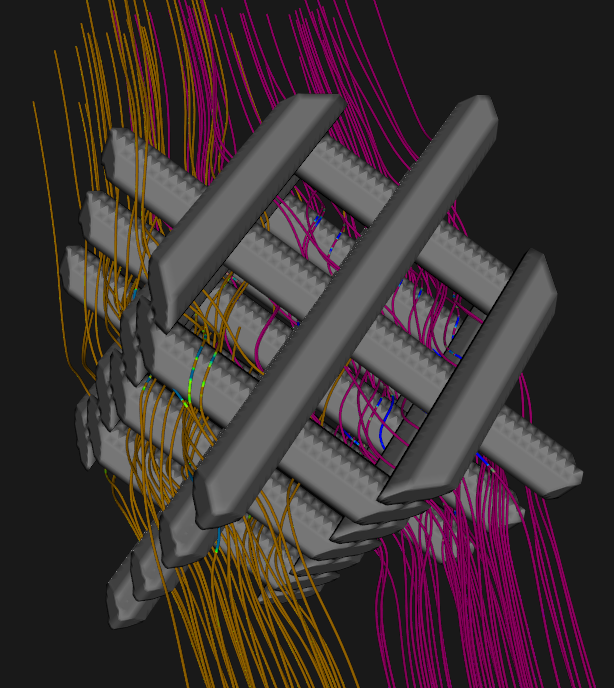
\includegraphics[width=\textwidth]{purple_yellow}
    \caption{Visualization}
    \label{fig:1}
\end{figure}


\end{document}
